\documentclass[11pt]{article}

    
    
    \usepackage{martins} % own defined packages in this file.

    

    
    
    % Document parameters
    % Document title
    \title{Ship power prediction}
    
    
    
    \author{Martin Alexandersson}
    
    
    

    
    
    
	
    

\begin{document}
    
    \maketitle
    
    

    
    \hypertarget{abstract}{%
\section{Abstract}\label{abstract}}

Short abstract of report

    \hypertarget{introduction}{%
\section{Introduction}\label{introduction}}

    

    \begin{figure}[H]
        \begin{center}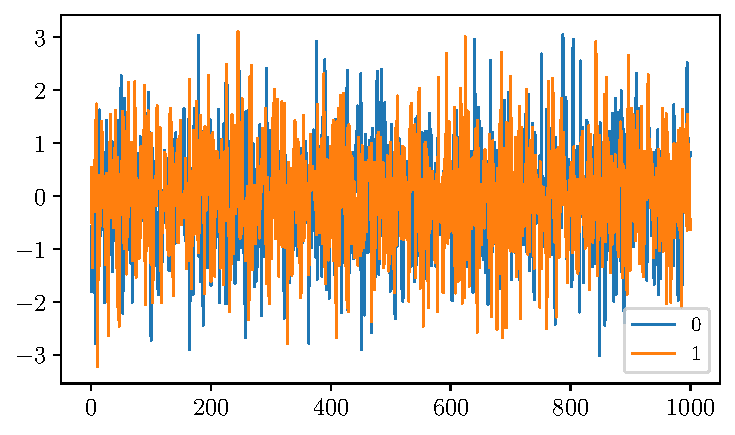
\includegraphics[width = 0.95\textwidth]{rolldecay_example.pdf}\end{center}
        \vspace{-0.7cm}
        \caption{Roll decay time series}
        \label{fig:rolldecay_example}
    \end{figure}
    
    The oscillating motion can be described by a spring-mass-damper system
as seen in Fig.Section \ref{fig_spring_mass_damper}.

    

    
    \begin{figure}[H]
        \begin{center}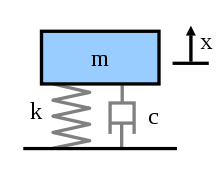
\includegraphics[width = 0.95\textwidth]{spring_mass_damper.png}\end{center}
        \vspace{-0.7cm}
        \caption{Spring-mass-damper system}
        \label{fig:spring_mass_damper}
    \end{figure}
    

    This system can me described as the following equation
Section \ref{eq_equation1}:

    

    
    $\displaystyle 
\begin{equation}
$E=m \dot c^2 $
\label{eq:equation1}
\end{equation}
$

    

    
    $\displaystyle 
\begin{equation}
A = \pi r^{2}
\label{eq:equation2}
\end{equation}
$

    

    \hypertarget{data}{%
\section{Data}\label{data}}

The data used in this study is described in
Tab.Section \ref{tab_data_files}. There is one result with a pure FNPF
simulation at 0 knots. For model test results, two tests are available
at 0 knots and one test at 15.5 knots. There is also a result at 15.5
with a hybrid method, where semi empirical viscosity has been injected
into the FNPF calculations.

    

    
    
\begin{table}[H]
\scriptsize
\center
\caption{Data files}
\label{tab:data_files}
\begin{tabular}{|l|l|l|l|}
\hline\addlinespace
file & data file & Ship speed & Method\\ 
 &  & $[kts]$ & \\ 
\hline1 & fnpf kvlcc2 rolldecay 0kn.csv & 0.0 & FNPF\\ 
2 & model test 21337.csv & 0.0 & model test\\ 
3 & model test 21338.csv & 0.0 & model test\\ 
4 & model test 21340.csv & 15.5 & model test\\ 
5 & fnpf kvlcc2 rolldecay 15-5kn ikeda dev.csv & 15.5 & hybrid\\ 

\hline
\end{tabular}
\end{table}

    

    \hypertarget{analysis}{%
\section{Analysis}\label{analysis}}

    \hypertarget{conclusions}{%
\section{Conclusions}\label{conclusions}}


    % Add a bibliography block to the postdoc
    
    
    
\end{document}
